% !TEX program = xelatex
\documentclass{article}
\usepackage[]{amsthm} %lets us use \begin{proof}
\usepackage{amsmath}
\usepackage{enumerate}
\usepackage{xparse}
\usepackage[makeroom]{cancel}
\usepackage[]{amssymb} %gives us the character \varnothing
\usepackage{fontspec}
\usepackage{polyglossia}
\usepackage{relsize}
\usepackage{graphicx}
\usepackage[left=2.0cm, top=2.0cm, right=2.0cm, bottom=2.0cm]{geometry}

\setdefaultlanguage{hebrew}
\setotherlanguage{english}

\setmainfont{[Arial.ttf]}
\newfontfamily\hebrewfont{[Arial.ttf]}

\newtheorem{lemma}{טענת עזר}

\title{מטלת מנחה 12 - אינפי 2}
\author{328197462}
\date{25/11/2022}

\begin{document}
\maketitle

\section*{שאלה 1}

נחשב את כל האינטגרלים

\subsection*{סעיף א}

\[
    \int \frac{x^5}{1-x^3}dx =
    \int \frac{x^2\cdot x^3 - x^2 + x^2}{1-x^3}dx =
    \int \frac{x^2(x^3 - 1) + x^2}{1-x^3}dx =
\]
\[
    \int (-x^2 - \frac{x^2}{x^3-1})dx =
    -\frac{x^3}{3} + \int \frac{(x^3-1)'}{x^3-1}dx =
    \begin{bmatrix}
        \mathsmaller{\text{לפי נגזרת}} \\
        \mathsmaller{\text{הפונקציה}}  \\
        \mathsmaller{\text{הלוגוריתמית}}
    \end{bmatrix} =
    -\frac{x^3}{3} + \ln(x^3-1) + C
\]

\subsection*{סעיף ב}

\[
    \int (3x-7)^4dx=
    [\mathsmaller{\mathsmaller{\int x^4dx=\frac{1}{5}x^5+C}}]=
    \frac{1}{3} \cdot \frac{(3x-7)^5}{5} + C =
    \frac{(3x-7)^5}{15} + C
\]

\subsection*{סעיף ג}

\[
    \int \frac{\sqrt{1+x^2} + \sqrt{1-x^2}}{\sqrt{1-x^4}}dx =
    \int \frac{\sqrt{1+x^2} + \sqrt{1-x^2}}{\sqrt{1+x^2} \cdot \sqrt{1-x^2}}dx =
    \int (\frac{1}{\sqrt{1-x^2}} + \frac{1}{\sqrt{1+x^2}})dx =
\]
\[
    \begin{bmatrix}
        \text{לפי דוגמה 2.29} \\
        \int \frac{1}{\sqrt{1+x^2}}dx = \ln|x+\sqrt{1+x^2}| + C
    \end{bmatrix}
    = \arcsin x + \ln|x+\sqrt{1+x^2}| + C
\]

\pagebreak

\subsection*{סעיף ד}

\[
    \int \frac{\sin x \cos x}{\sin ^2 x + \sin x + 1}dx=
    \begin{bmatrix}
        t=\sin x \\
        dt=\cos x dx
    \end{bmatrix} =
    \int \frac{tdt}{t^2+t+1}=
    \begin{bmatrix}
        \mathsmaller{t=\frac{1}{2}(2t+1) - \frac{1}{2}}
    \end{bmatrix} =
    \frac{1}{2} \int \frac{(2t+1)dt}{t^2+t+1} - \frac{1}{2} \int \frac{dt}{t^2+t+1}
\]
כאשר לפי הצבה לוגוריתמית \[
    \int \frac{(2t+1)dt}{t^2+t+1} =
    \ln(t^2+t+1) + C
\]
וכן, \[
    \int \frac{dt}{t^2+t+1} =
    \int \frac{dt}{(t+0.5)^2+0.75}=
    \mathsmaller{
        \begin{bmatrix}
            u=t+0.5 \\
            du=dt
        \end{bmatrix}
    } =
    \int \frac{du}{u^2+0.75}=
\]
\[
    \mathsmaller{
        \begin{bmatrix}
            \text{שאלה 7ב ביחידה 2} \\
            a^2 = \frac{3}{4}       \\
            a = \frac{\sqrt{3}}{2}
        \end{bmatrix}
    } =
    \frac{2}{\sqrt{3}}\arctan \frac{2u}{\sqrt{3}} + C =
    \frac{2\sqrt{3}}{3}\arctan \frac{2\sqrt{3}(t+0.5)}{3} + C =
    \frac{2\sqrt{3}}{3}\arctan \frac{2\sqrt{3}t+\sqrt{3}}{3} + C
\]
ומכאן נקבל \[
    \int \frac{tdt}{t^2+t+1}=
    \frac{1}{2} \int \frac{(2t+1)dt}{t^2+t+1} - \frac{1}{2} \int \frac{dt}{t^2+t+1} =
    \frac{1}{2} \ln(t^2+t+1) - \frac{\sqrt{3}}{3}\arctan \frac{2\sqrt{3}t+\sqrt{3}}{3} + C
\]
ולכן \[
    \int \frac{\sin x \cos x}{\sin ^2 x + \sin x + 1}dx=
    \frac{1}{2} \ln(\sin^2x+\sin x+1) - \frac{\sqrt{3}}{3}\arctan \frac{2\sqrt{3}\sin x+\sqrt{3}}{3} + C
\]

\subsection*{סעיף ה}

\[
    \int \frac{e^{2x}}{16+e^{4x}}dx =
    \begin{bmatrix}
        t=e^{2x}     \\
        dt=2e^{2x}dx \\
        \frac{1}{2} dt = e^{2x}dx
    \end{bmatrix} =
    \frac{1}{2} \cdot \int \frac{dt}{16+t^2}=
\]
\[
    \begin{bmatrix}
        \text{שאלה 7ב ביחידה 2} \\
        a^2=16                  \\
        a=4
    \end{bmatrix} =
    \frac{1}{8} \arctan \frac{t}{4} + C =
    \frac{1}{8} \arctan \frac{e^{2x}}{4} + C
\]

\subsection*{סעיף ו}

\[
    \int \frac{\arcsin x}{\sqrt{x+1}}dx =
    \begin{bmatrix}
        u=\arcsin x               & v'=(x+1)^{-\frac{1}{2}}  \\
        u'=\frac{1}{\sqrt{1-x^2}} & v= 2 (x+1)^{\frac{1}{2}}
    \end{bmatrix} =
    2\arcsin x \cdot \sqrt{x+1} - \int \frac{1}{\sqrt{1-x^2}} \cdot 2\sqrt{x+1}dx =
\]
כאשר מתקיים: \[
    \int \frac{1}{\sqrt{1-x^2}} \cdot 2\sqrt{x+1}dx =
    2 \int \frac{1}{\sqrt{1-x}} dx=
    2 \int (1-x)^{-\frac{1}{2}}dx =
    2 \cdot 2(1-x)^{\frac{1}{2}}\cdot (-1) + C =
    -4\sqrt{1-x} + C
\]
ולכן \[
    \int \frac{\arcsin x}{\sqrt{x+1}}dx =
    2\arcsin x \cdot \sqrt{x+1} - \int \frac{1}{\sqrt{1-x^2}} \cdot 2\sqrt{x+1}dx =
    2\arcsin x \cdot \sqrt{x+1} + 4\sqrt{1-x} + C
\]

\subsection*{סעיף ז}

\[
    \int \ln(x^2-3x+2)dx=
    \int \ln(x^2-3x+2)\cdot 1dx=
    \begin{bmatrix}
        u=\ln(x^2-3x+2)          & v'=1 \\
        u'=\frac{2x-3}{x^2-3x+2} & v=x
    \end{bmatrix}=
    x\ln(x^2-3x+2) - \int \frac{2x-3}{x^2-3x+2} \cdot xdx
\]
כאשר מתקיים \[
    \int \frac{2x-3}{x^2-3x+2} \cdot xdx =
    \int \frac{2x^2-3x}{x^2-3x+2}dx
\]
נרצה לבצע חילוק פולינומים על מנת להעביר את האינטגרל לצורה פשוטה יותר. \\
שורשי המכנה הם $x=1,2$, לכן נרצה להעביר את האינטגרד לצורה $\frac{a}{x-1} + \frac{b}{x-2} + p(x)$ כאשר $p$ פולינום

נפתור את מערכת המשוואות ע"י כפל במכנה\[
    \frac{2x^2-3x}{x^2-3x+2} = \frac{a}{x-1} + \frac{b}{x-2} + p(x)
    \xrightarrow{\cdot (x-1)(x-2)}
    2x^2-3x=a(x-2)+b(x-1) + p(x)(x^2-3x+2)
\]
נקבל כי מעלת הפולינום $p$ היא לכל היותר 1, שכן אחרת מעלת הביטוי מימין תהיה גבוהה ממעלת הביטוי משמאל.\\
נסמן $p(x) = k$
\[
    \Rightarrow \begin{cases}
        [x^2]: 2=k                             \\
        [x]: -3=a+b-3k=a+b-6 \Rightarrow a+b=3 \\
        [1]: 0= -2a-b+2k=-2a-b+4 \Rightarrow 2a + b = 4
    \end{cases}
\]
נחסר את שתי המשוואות האחרונות זו מזו ונקבל $a=1\Rightarrow b=2$ \\
לכן פונקציית האינטגרד היא $\frac{1}{x-1} + \frac{2}{x-2} + 2$ \\
ונקבל: \[
    \int \frac{2x^2-3x}{x^2-3x+2}dx =
    \int \frac{1}{x-1}dx + 2 \int \frac{1}{x-2}dx + \int 2dx =
    \ln(x-1) + 2\ln(x-2) + 2x + C
\]

לסיכום: \[
    \int \ln(x^2-3x+2)dx =
    x\ln(x^2-3x+2) - \ln(x-1) -2\ln(x-2) - 2x + C
\]

\pagebreak

\section*{שאלה 2}

\subsection*{סעיף א}

\[
    \int_0^{\pi/3} \frac{dx}{5-4\cos x} =
    \begin{bmatrix}
        t=\tan\frac{x}{2}            \\
        \cos x = \frac{1-t^2}{1+t^2} \\
        dx = \frac{2}{1+t^2}dt       \\
        \text{לפי 2.3.8}             \\
        x=0,\pi/3 \Rightarrow t=0,\sqrt{3}/3
    \end{bmatrix} =
    \int_0^{\sqrt{3}/3} \frac{1}{5-4(\frac{1-t^2}{1+t^2})} \cdot \frac{2}{1+t^2}dt =
\]
\[
    \int_0^{\sqrt{3}/3} \frac{1+t^2}{5(1+t^2)-4(1-t^2)} \cdot \frac{2}{1+t^2}dt =
    2 \int_0^{\sqrt{3}/3} \frac{dt}{5+t^2-4+4t^2} =
    2 \int_0^{\sqrt{3}/3} \frac{dt}{9t^2+1} =
    \frac{2}{9} \int_0^{\sqrt{3}/3} \frac{dt}{t^2+(\frac{1}{3})^2} =
\]
\[
    \begin{bmatrix}
        \text{לפי שאלה 7ב} \\
        \text{ביחידה 2}
    \end{bmatrix} =
    \frac{2}{9} \cdot 3\arctan 3t \bigg|_0^{\sqrt{3}/3} =
    \frac{2\pi}{9}
\]

\subsection*{סעיף ב}

נתחיל בחישוב פונקציה קדומה לפונקציית האינטגרד. \\
נתקלנו בפונקציה קדומה מהצורה $\int \frac{P(x)}{Q(x)\sqrt{ax^2+bx+c}}dx$,
לכן נבצע הצבת אוילר: $\sqrt{x^2+1}=t-x$

נקבל, לפי עמוד 161
\[
    x=\frac{t^2-1}{2t} ; \;
    dx = \frac{t^2+1}{2t^2}dt ; \;
    x+1 = \frac{t^2-1}{2t}+\frac{2t}{2t} = \frac{t^2+2t-1}{2t} \;
    \sqrt{x^2+1}=t\cdot \frac{2t}{2t}-\frac{t^2-1}{2t}=\frac{t^2+1}{2t}
\]
נשים לב בנוסף: $x=0\Rightarrow t=1, x=1 \Rightarrow t=\sqrt{2}+1$

ומכאן:
\[
    \int_0^1 \frac{dx}{(x+1)\sqrt{x^2+1}} =
    \int_1^{\sqrt{2}+1} \frac{1}{\frac{t^2+2t-1}{2t} \cdot \frac{t^2+1}{2t}} \cdot \frac{t^2+1}{2t^2}dt =
    \int_1^{\sqrt{2}+1} \frac{4t^2}{2t^2(t^2+2t-1)}dt =
    2 \int_1^{\sqrt{2}+1} \frac{dt}{t^2+2t-1}
\]

נרצה להפריד לצורת $\frac{a}{t-(-1+\sqrt{2})} + \frac{b}{t-(-1-\sqrt{2})}$.
\[
    \frac{1}{t^2+2t-1}=\frac{a}{t+1-\sqrt{2}} + \frac{b}{t+1+\sqrt{2}}                                \\
\]
\[
    1=a(t+1+\sqrt{2}) + b(t+1-\sqrt{2})
\]
נשווה מקדמים של איברי הפולינום:
\[
    \begin{cases}
        [t] \; a+b=0 \; \Rightarrow a=-b \\
        [1] \; a+\sqrt{2}a+b-\sqrt{2}b=1 \; \Rightarrow 2\sqrt{2}a=1
    \end{cases}
\]
נקבל $a=\frac{1}{2\sqrt{2}}, b=-\frac{1}{2\sqrt{2}}$

\[
    2 \int_1^{\sqrt{2}+1} \frac{dt}{t^2+2t-1} =
    \frac{1}{\sqrt{2}} \int_1^{\sqrt{2}+1}
    (\frac{1}{t+1-\sqrt{2}} - \frac{1}{t+1+\sqrt{2}})dt =
    \frac{1}{\sqrt{2}} (\ln(\frac{t+1-\sqrt{2}}{t+1+\sqrt{2}})\bigg|_1^{\sqrt{2}+1}) =
\]
\[
    \frac{1}{\sqrt{2}} (\ln(\frac{2}{2+2\sqrt{2}}) - \ln(\frac{2-\sqrt{2}}{2+\sqrt{2}})) =
    \frac{1}{\sqrt{2}} \ln(\frac{2}{2-\sqrt{2}})\approx 0.868
\]

\pagebreak

\subsection*{סעיף ג}

נשתמש בתכונת הלינאריות של האינטגרל

\[
    \int_{-\pi/4}^{\pi/4} \frac{x^7-x+1}{\cos^2x}dx =
    \int_{-\pi/4}^{\pi/4} \frac{x^7-x}{\cos^2x}dx + \int_{-\pi/4}^{\pi/4} \frac{1}{\cos^2x}dx =
    \int_{-\pi/4}^{\pi/4} \frac{x^7-x}{\cos^2x}dx + \tan x\bigg|_{-\pi/4}^{\pi/4}
\]

באשר לאינטגרל שנותר, נשים לב כי פונקציית האינטגרד $f(x) = \frac{x^7-x}{\cos^2x}$ היא אי-זוגית. המונה הוא פונקציית פולינום אי-זוגית, והמכנה הוא פונקציה זוגית ידועה, וביחד המנה תהיה אי-זוגית.\\
לכן ניעזר בשאלה 43 ביחידה 2. נקבל $\int_{-\pi/4}^{\pi/4} f(x)dx = 0$

ולסיכום:
\[
    \int_{-\pi/4}^{\pi/4} \frac{x^7-x+1}{\cos^2x}dx =
    0 + \tan x\bigg|_{-\pi/4}^{\pi/4} =
    0 + 1 - (-1) = 2
\]


\subsection*{סעיף ד}
נשתמש בתכונת האדיטיביות של האינטגרגל $\int_0^5 ||x-1|-|x-2||dx$
\[
    \int_0^5 ||x-1|-|x-2||dx =
    \int_0^1 ||x-1|-|x-2||dx + \int_1^2 ||x-1|-|x-2||dx + \int_2^5 ||x-1|-|x-2||dx
\]
בתחום $[0,1]$ נקבל $x\leq 1,2\Rightarrow |x-1|=-x+1, |x-2|=-x+2$ \\
ולכן האינטגרד בתחום זה יהיה $||x-1|-|x-2||=|-x+1-((-x)+2)|=|-1|=1$ \\
ונקבל: \[
    \int_0^1 ||x-1|-|x-2||dx =
    \int_0^1 1dx =
    x\bigg|_0^1 =
    1 - 0 = 1
\]

באופן דומה: \[
    \int_1^2 ||x-1|-|x-2||dx =
    \int_1^2 |x-1-(-x+2)|dx =
    \int_1^2 |2x-3|dx =
\]
\[
    \int_1^{1.5} (-2x+3)dx + \int_{1.5}^2 (2x-3)dx =
    (-x^2+3x)\bigg|_1^{1.5} + (x^2-3x)\bigg|_{1.5}^2 =
    -\frac{27}{4} - (-4) + 10 - \frac{27}{4} =
    \frac{1}{2}
\]
וכן \[
    \int_2^5 ||x-1|-|x-2||dx =
    \int_2^5 |(x-1)-(x-2)|dx =
    \int_2^5 |1|dx =
    x\bigg|_2^5 =
    5 - 2 = 3
\]
לסיכום נקבל \[
    \int_0^5 ||x-1|-|x-2||dx =
    1 + \frac{1}{2} + 3 =
    4.5
\]

\pagebreak

\section*{שאלה 3}

\subsection*{סעיף א}

הטעות טמונה במעבר
$\int_1^{1+2\pi}\cos x \cdot e^{-\sin^2x}dx =
    \int_{\sin 1}^{\sin 1}e^{-t^2}dt$. \\
השתמשנו כאן במשפט $2.11$. לפי המשפט, מתקיים השוויון הבא:
\[
    \int_{\sin 1}^{\sin 1}f(x)dx=\int_1^{1+2\pi} f(\sin(t)) \cos x dt
\]
כאשר $f(x) = e^{-x^2}$,
זאת בכפוף לתנאי המשפט. \\
אכן, $\sin$
מוגדרת בקטע $[1, 1+2\pi]$
כנדרש בתנאי הראשון. \\
התנאי השני של במשפט דורש $\sin([1, 1+2\pi])\subseteq [\sin 1, \sin 1] = \{\sin 1\}$
נשים לב כי מדובר במחזור שלם של פונקציית הסינוס, ולכן $\sin([1, 1+2\pi])=[-1,1]$
והתנאי לא מתקיים! זוהי הטעות בהצבה.

\subsection*{סעיף ב}

ניעזר בתכונת האדיטויביות של האינטגרל:
\[
    I=
    \int_1^{1+2\pi}\cos x \cdot e^{-\sin^2x}dx =
    \int_1^{1+\pi}\cos x \cdot e^{-\sin^2x}dx +
    \int_{1+\pi}^{1+2\pi}\cos x \cdot e^{-\sin^2x}dx
\]

נחשב את ערך האינטגרל $\int_{1+\pi}^{1+2\pi}\cos x \cdot e^{-\sin^2x}dx$
כעת נציב $t=x-\pi$. \\
אז $dt=dx$, ונקבל:
\[
    \int_{1+\pi}^{1+2\pi}\cos x \cdot e^{-\sin^2x}dx =
    \begin{bmatrix}
        x = 1 + \pi  & \Rightarrow & t =  1      \\
        x = 1 + 2\pi & \Rightarrow & t = 1 + \pi
    \end{bmatrix} =
    \int_1^{1+\pi} \cos (t+\pi) \cdot e^{-\sin^2(t+\pi)}dt
\]

כעת, ניעזר בזהויות טריגונומטריות מאינפי 1:
\[
    \sin(t+\pi) = -\sin(2\pi - (t+\pi)) = -\sin (\pi - t) = -\sin t
    \Rightarrow -\sin^2(t+\pi) = -(-\sin t)^2 =-\sin t
\]
\[
    \cos(t+\pi) = \cos (2\pi - (t+\pi)) = \cos (\pi - t) = -\cos t
\]

נקבל:
\[
    \int_{1+\pi}^{1+2\pi}\cos x \cdot e^{-\sin^2x}dx =
    \int_1^{1+\pi} \cos (t+\pi) \cdot e^{-\sin^2(t+\pi)}dt =
    -\int_1^{1+\pi} \cos t \cdot e^{-\sin^2t}dt
\]

ולכן
\[
    I =
    \int_1^{1+\pi}\cos x \cdot e^{-\sin^2x}dx +
    \int_{1+\pi}^{1+2\pi}\cos x \cdot e^{-\sin^2x}dx =
\]
\[
    =\int_1^{1+\pi}\cos x \cdot e^{-\sin^2x}dx -
    \int_1^{1+\pi}\cos x \cdot e^{-\sin^2x}dx =
    0
\]

\pagebreak

\section*{שאלה 4}

נסמן לפי הנתון, לכל $n\in \mathbb{N}$:
\[
    \begin{matrix}
        S_n = \int \sin ^n(x) dx &
        C_n = \int \cos ^n(x) dx
    \end{matrix}
\]

לכל $n\geq 3$
טבעי:
\[
    S_n = \int \sin^n(x)dx =
    \int \sin ^2 (x) \cdot \sin ^{n-2}(x) dx =
    \int (1-\cos^2x) \cdot \sin ^{n-2}(x) dx =
    S_{n-2} - \int \cos ^2 x \cdot \sin ^{n-2}(x) dx
\]
נבצע אינטגרציה בחלקים למחוסר. נקבל:
\[
    \int \cos ^2 x \cdot \sin ^{n-2}(x) dx =
    \begin{bmatrix}
        u=\cos x   &
        v'=\cos x \cdot \sin^{n-2}(x) \\
        u'=-\sin x &
        v = \frac{1}{n-1}\cdot \sin^{n-1}(x)
    \end{bmatrix} =
    \frac{1}{n-1} \cos x \cdot \sin^{n-1}(x) - \frac{1}{n-1} \int -\sin^n(x)dx
\]
נשים לב:
$-\frac{1}{n-1} \int -\sin^n(x)dx = \frac{1}{n-1} S_n$.
לכן נעביר אגפים ונקבל:
\[
    \frac{n-1}{n-1} S_n = S_{n-2} - \frac{1}{n-1} \cos x \cdot \sin^{n-1}(x) - \frac{1}{n-1} S_n
\]
\[
    \frac{n}{n-1}S_n = - \frac{1}{n-1} \cos x \cdot \sin^{n-1}(x) + S_{n-2}
\]
\[
    S_n = - \frac{1}{n} \cos x \cdot \sin^{n-1}(x) + \frac{n-1}{n} S_{n-2}
\]
ובכך הוכחנו את הנוסחה הראשונה.
\\\\
נעבור לנוסחה השנייה ונחזור על התהליך בקצרה. \\
\[
    C_n = C_{n-2} - \int \sin^2x\cdot \cos^{n-2}(x)dx
\]
\[
    \int \sin^2x\cdot \cos^{n-2}(x)dx =
    \begin{bmatrix}
        u=\sin x  &
        v'=\sin x \cdot \cos^{n-2}(x) \\
        u'=\cos x &
        v = \frac{-1}{n-1}\cdot \cos^{n-1}(x)
    \end{bmatrix} =
    \frac{-1}{n-1} \sin x \cdot \cos^{n-1}(x) + \frac{1}{n-1} C_n
\]
\[
    \frac{n-1}{n-1} C_n = C_{n-2} + \frac{1}{n-1} \sin x \cdot \cos^{n-1}(x) - \frac{1}{n-1} C_n
\]
\[
    \frac{n}{n-1}C_n = - \frac{1}{n-1} \sin x \cdot \cos^{n-1}(x) + C_{n-2}
\]
\[
    C_n = \frac{1}{n} \sin x \cdot \cos^{n-1}(x) + \frac{n-1}{n} C_{n-2}
\]

\pagebreak

\section*{שאלה 5}

נרצה לחשב את השטח המוגבל על ידי העקומה $y^2=(1-x^2)^3$. \\
ראשית, על מנת שהעקומה תהא מוגדרת, נדרוש $(1-x^2)^3\geq 0$.
נקבל $1-x^2\geq 0$,
ולכן $-1\leq x \leq 1$
\\\\
לכל $x\in[-1,1]$,
נקבל שני ערכי $y$,
והם $y=\pm \sqrt{(1-x^2)^3}$. השטח המוגבל שנרצה לחשב ייראה כך:

\begin{figure}[h]
    \centering
    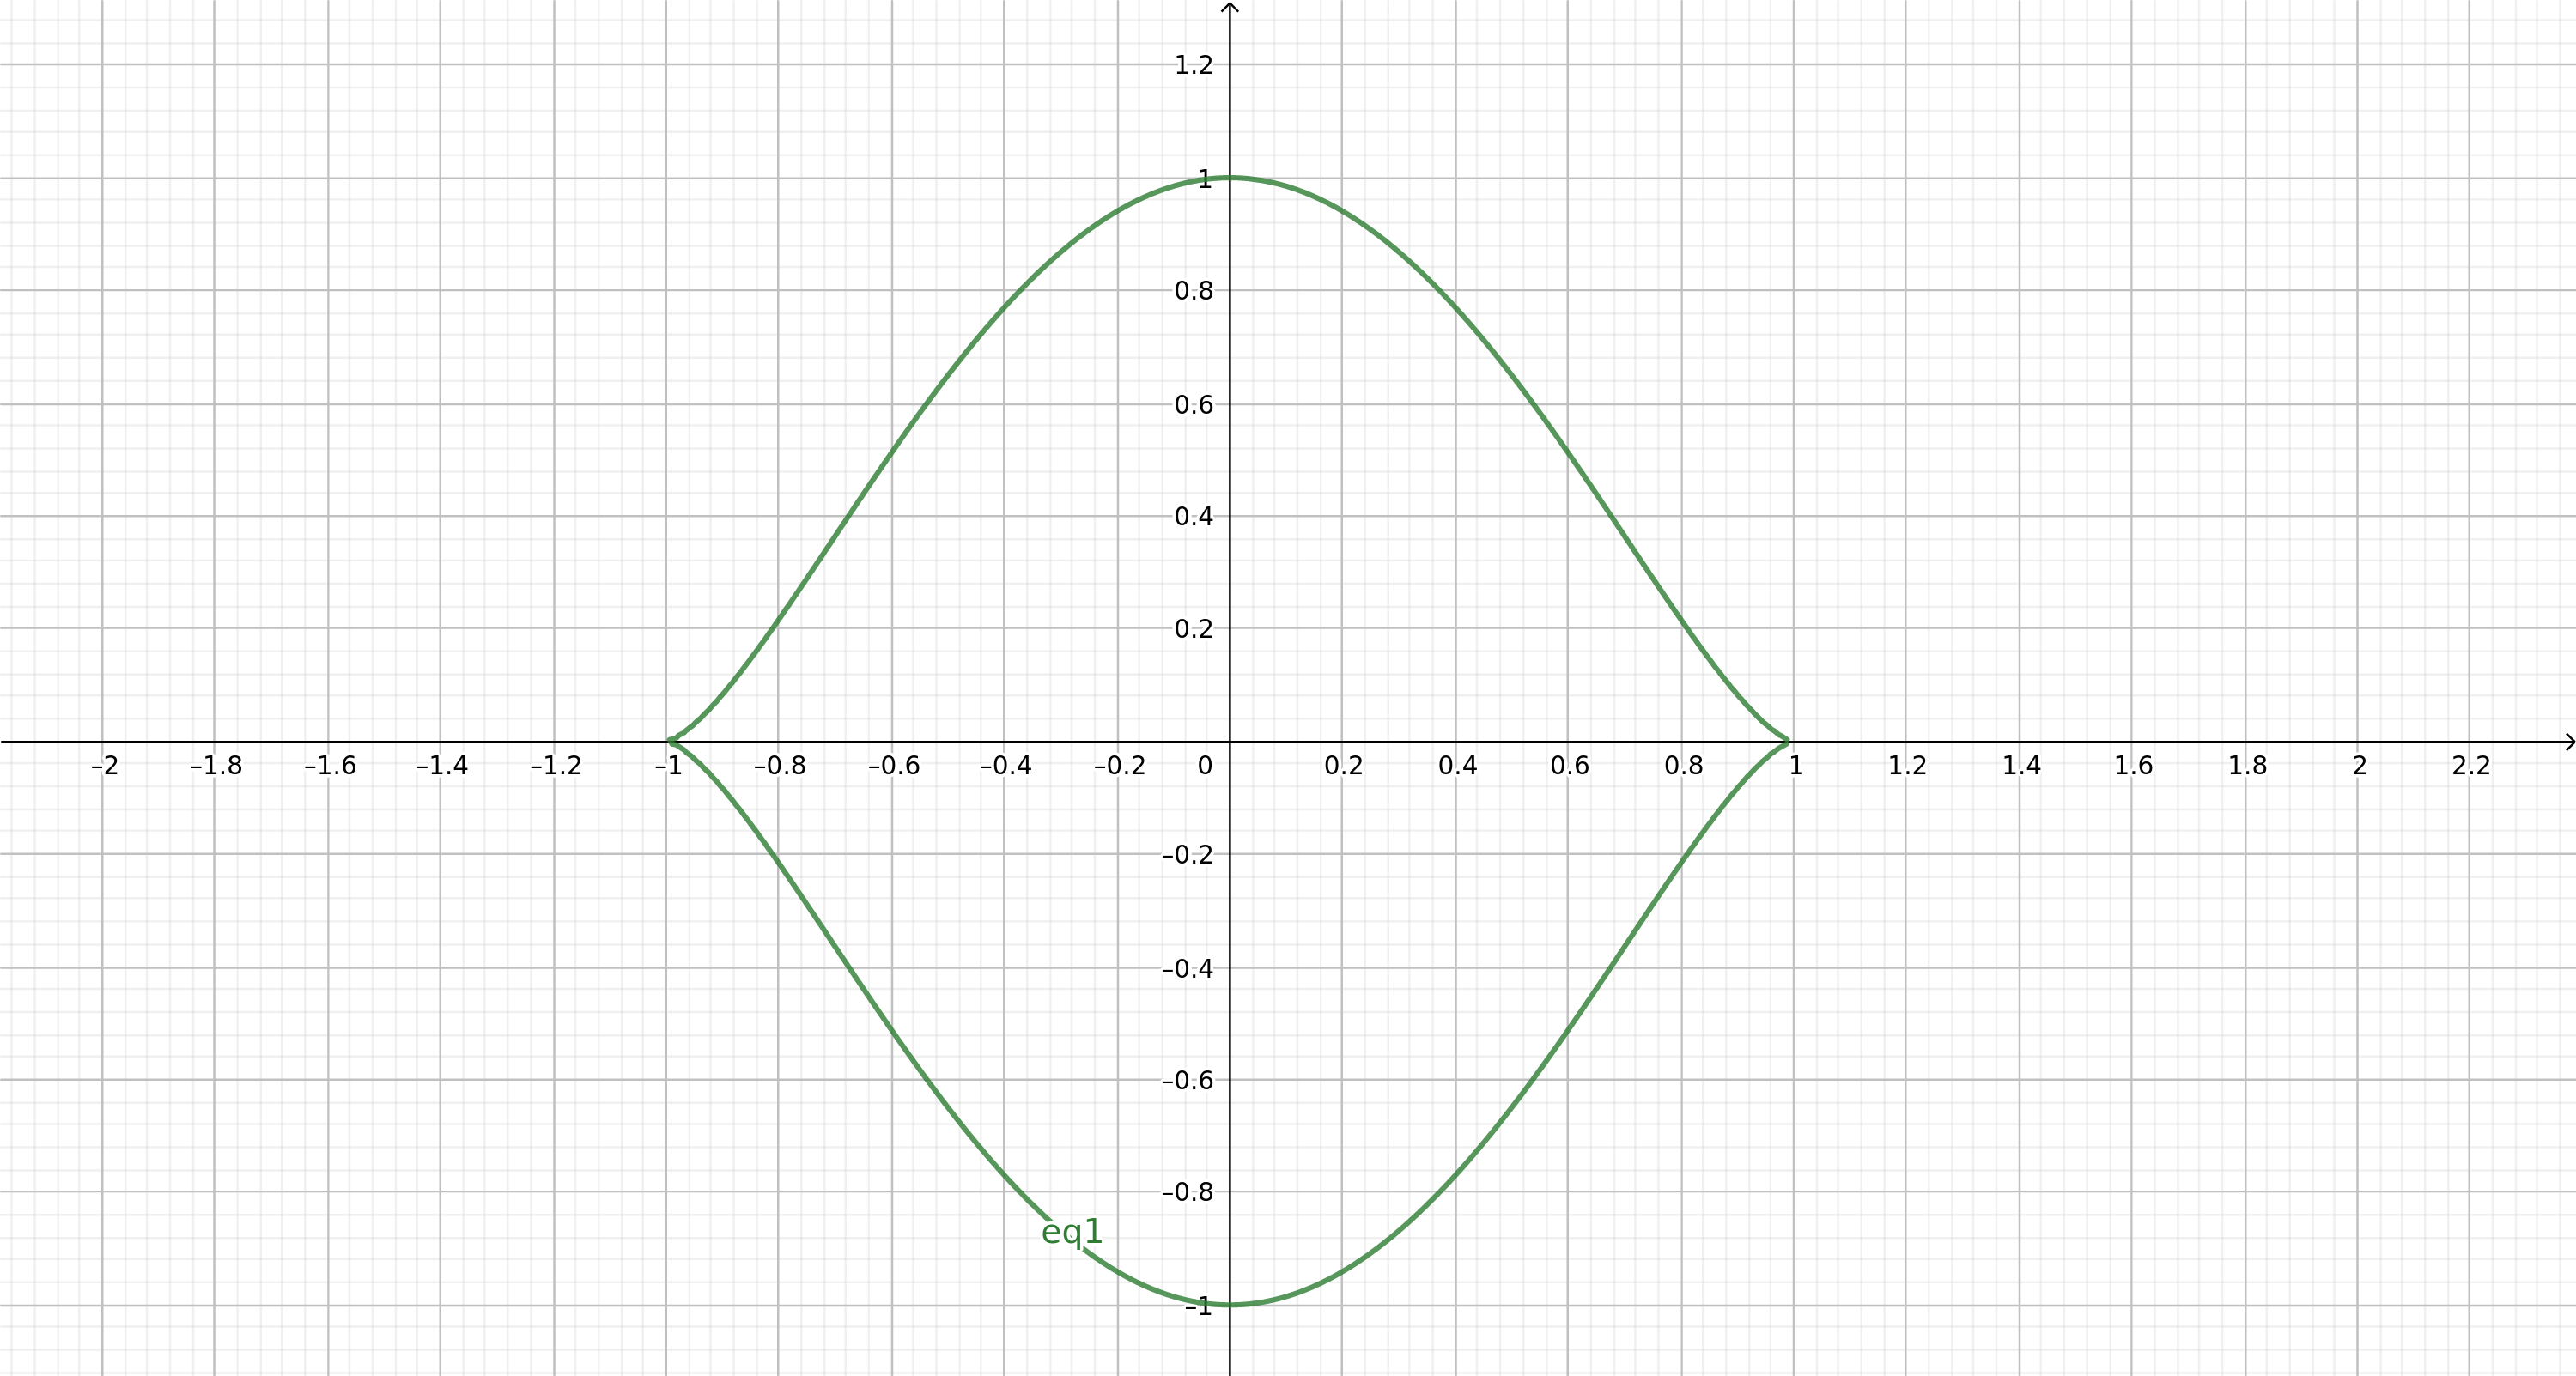
\includegraphics[width=0.7\linewidth]{20475-assignment-12-05-graph.png}
\end{figure}

נשים לב כי השטח סימטרי ביחס לציר ה $x$.
אכן, לכל $x\in[-1,1]$ נקבל:
\[
    y(-x) = \pm \sqrt{(1-(-x)^2)^3} = \pm \sqrt{(1-x^2)^3} = y(x)
\]
על כן, השטח שלנו יהיה, לפי דוגמה $1.17$:
\[
    S=\int_{-1}^1 (\sqrt{(1-x^2)^3} - (-\sqrt{(1-x^2)^3}))dx =
    2 \int_{-1}^1 \sqrt{(1-x^2)^3}dx =
    [\text{משיקולי סימטריה}] =
    4 \int_0^1 \sqrt{1-x^2}^3dx
\]

כעת נציב $x=\sin t$,
אז $dx=\cos t dt$
ונקבל:
\[
    4\int_0^1 \sqrt{1-x^2}^3dx =
    \begin{bmatrix}
        x=0\Rightarrow t=0     \\
        x=1\Rightarrow t=\pi/2 \\
    \end{bmatrix} =
    4\int_0^{\pi/2} \sqrt{1-\sin^2t}^3\cdot \cos t dt =
    \begin{bmatrix}
        \text{בתחום המבוקש מתקיים} \\
        \cos t = \sqrt{1-\sin^2t}
    \end{bmatrix} =
    4 \int_0^{\pi/2} \cos^4t dt
\]
משאלה 4 נקבל $\int \cos^4 x dx = \frac{1}{4}\sin x \cdot \cos^3x + \frac{3}{4} \int \cos^2xdx$

\end{document}